 \section{Multi Label Learning}
 
\subsection*{Introduction}
\begin{frame}{Multi label classification}
	Motivation:
	\begin{itemize}\setlength\itemsep{1em}
		\item Sometimes a complex item can be well represented by a set of \textit{labels}
		\item Helps single label classification when the concept is more complicated or general
	\end{itemize}
	Solutions:
	\begin{itemize}\setlength\itemsep{1em}
		\item Problem transformation
		\item Algorithm adaptation
	\end{itemize}
\end{frame}

\begin{frame}{Notation}
	A set of labels $L = \{y_1, y_2,... y_l\}$ is given.\\
	Each object contained in the dataset is associated with a set of labels:
	\begin{columns}
		\begin{column}{0.5\textwidth}\centering
		$$D = \{(X_i, Y_i | i \in [1, n]\}$$
		$$X_i \in \R^f$$
		$$Y_i = \{y_{i,h} | h \in [1, h_i], y_{i,h} \in L, h_i \leq l\}$$
		\end{column}
		\begin{column}{0.5\textwidth}\centering
		\begin{figure}[htbp]
			\centering
			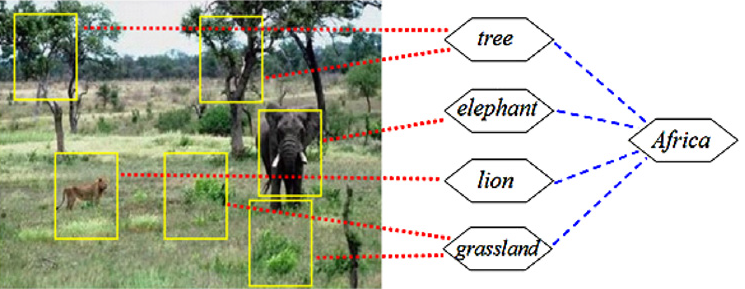
\includegraphics[scale = 0.3]{./images/ml1.png}
			\caption{\textit{Multi label example}}
		\end{figure}
		\end{column}
	\end{columns}
	
	
	\color{red}IMMAGINE ML?
	
\end{frame}

\begin{frame}{Problem transformation}
	Attempt to convert the multilabel problem in a regular binary task.
	
	Two lossy methods:
	\begin{itemize}\setlength\itemsep{1em}
		\item Randomly discard each label information except one from each instance
		\item Remove instances that have actually more than one label
	\end{itemize}
	Other solutions:
	\begin{itemize}\setlength\itemsep{1em}
		\item Train a binary classifier for each existing combination of labels
		\item Train a binary classifier for each label (used in this work)
	\end{itemize}
\end{frame}

\begin{frame}{Algorithm adaptation}
	Regular algorithms are modified to support multi-label tasks.
	
	Sometimes they use problem transformation at the core.
	
	An example using SVM-related approach based on ranking and label set size prediction.
	
	\color{red}???
\end{frame}

\begin{frame}{Another multi label approch}
	
	\begin{flushright}
		\cite{ml1}
	\end{flushright}
\end{frame}